%Artigo escrito por Anderson Vieira do Nascimento%
%Estudante de Cíência da Computação do IFB - 171057600005%

\documentclass[11pt]{article}
\usepackage[brazil]{babel}
\usepackage[utf8]{inputenc}
\usepackage[T1]{fontenc}
\usepackage[section]{placeins}
\usepackage{indentfirst}
\usepackage{graphicx}
\usepackage{amsmath}
\usepackage{amssymb}
\usepackage{textcomp}
\usepackage{gensymb}
\usepackage{hyperref}
\usepackage{wrapfig}

\usepackage{floatrow}
\newfloatcommand{capbtabbox}{table}[][\FBwidth]

\graphicspath{{./img/}}

\begin{document}

\title{Spline Cúbico Natural}
\author{Anderson Vieira do Nascimento}
\date{14/11/2018}
\maketitle

\section*{Resumo}

O objetivo do trabalho é explorar as capacidades
da interpolação de dados para a aproximação de silhuetas
por meio do uso de polinômios interpoladores conhecidos como
\textit{splines}. Com ``silhuetas'' queremos dizer que, a partir de imagens
escolhidas previamente, coletamos dados (os
pontos no plano cartesiano) das bordas das figuras escolhidas e, com uma
técnica de interpolação, aproximamos a curva gerada da forma
traçada pelos dados.

Para esse fim, implementamos a técnica em três figuras, sendo uma
delas mais explicitada na seção ``Resultados'' e as restantes apenas
exemplificadas na mesma seção. Os programas estão implementados em
Python 3.6, algumas figuras presentes no trabalho foram produzidas
no software GeoGebra e em outros aplicativos.

Ao final da exposição, são feitas observações a respeito da técnica, 
conclusões e considerações finais referentes aos resultados obtidos.

\section{Introdução}

Em diversas áreas da pesquisa científica há a necessidade
de identificar padrões de resultados numéricos em dados
coletados durante procedimentos de pesquisa. Uma das formas de obter esses padrões,
em termos de análise numérica, é a partir da interpolação. Existem várias
técnicas para esse tipo de aproximação de dados, tais como o
método de Newton, método Lagrange e interpolação por sistemas lineares [1]. 
Entretanto, em boa parte desses métodos há o problema do mau condicionamento 
das informações, o que pode acarretar em aproximações não esperadas.

Quando fazemos referência a esse aspecto dos dados, queremos dizer que
a inclinação obtida a partir de uma reta traçada entre dois pontos coletados
assume um valor alto. Como exemplo, considere os pontos
$P_0 = (1, 1)$, $P_1 = (0.0001, 10000)$ e tracemos uma reta entre eles.
A inclinação obtida é dada pela equação $tan(\theta) = 10000$, onde
$\theta \approx 1.57 \ rad \approx 89.99 \degree$. Esse valor alto de inclinação
pode ocasionar o aumento no erro da interpolação, dependendo do método
utilizado.

Para esses casos de mau condicionamento, o método de interpolação
por \textit{splines} é útil, pois ao invés de considerar todo
o intervalo fornecido (do ponto mais à esquerda ao ponto mais à direita),
ele considera cada par de pontos como o intervalo a ser utilizado para o traçamento
da curva que interpola os valores.

\subsection{\textit{Splines} e suas variações}

De acordo com o dicionário Thesaurus[2], um \textit{spline} é um
pedaço de madeira ou borracha, suficientemente flexível, utilizado
para desenhar curvas. Se pensarmos no contexto de interpolação de
dados, seria uma forma de forçar esse equipamento a se encaixar nos
pontos que queremos, de forma a nos possibilitar o traçamento de uma
curva.

De uma maneira geral, os \textit{splines} utilizam várias
funções para interpolar os valores em um dado intervalo, ou seja,
é uma interpolação por partes. Nesse trabalho, discutiremos \textit{splines}
que utilizam funções lineares (\textit{spline} linear) e funções cúbicas
(\textit{spline} cúbico natural ou fixado)[3], sendo a implementação focada
em \textit{spline} natural cúbico.

Em uma sequência de pontos, se utilizarmos funções lineares para interpolar
os valores entre cada par de pontos, o resultado pode não ser o
esperado.

Como exemplo, observe o gráfico da função $f(x) = \frac{1}{x}$ no intervalo
$[1, 6]$:

\begin{figure}[h]
\caption{$f(x) = \frac{1}{x}$}
\includegraphics[width=0.7\textwidth]{fig1_1}
\centering
\end{figure}

Agora, vamos montar um conjunto $P$ de pontos onde a função está definida:

$$P = {(1, 1), (1.3, 0.77), (2.5, 0.4), (3.2, 0.31), (5.1, 0.20), (6, 0.17)}$$

Utilizando o \textit{spline} linear para interpolar os pontos (ou apenas
ligá-los), obtemos o seguinte gráfico:

\begin{figure}[h]
\caption{Interpolação por \textit{spline} linear}
\includegraphics[width=0.7\textwidth]{fig1_2}
\centering
\end{figure}

De fato, o gráfico gerado lembra o gráfico da função $f(x) = \frac{1}{x}$ na
figura 1, mas como fazer uma interpolação de forma que no encontro de dois
pontos seja possível diferenciar a função? Em outras palavras, seja $S(x)$ a
nossa curva interpoladora, como igualar $S'(x_k)$ e $S'(x_{k+1})$, para 
$k = 0, 1, 2, 3, ..., n-1$? Ao responder esse questionamento, daremos um passo
importante para aproximar a nossa curva da função $f(x) = \frac{1}{x}$.

Esse ``equilíbrio'' das derivadas é garantido pelo \textit{spline} cúbico, pois
sendo $S(x)$ uma função cúbica (ou melhor, uma curva dividida em várias funções
cúbicas que chamaremos de $s_k(x)$ para $k = 1, 2, ..., n$), temos que, sendo $C$
uma constante tal que $C = 0$ ou $C \neq 0$, $s_k'(x) \neq C$, $s_k''(x) \neq C$,
o que garante certa suavidade para a curva que estamos analisando.  

Uma interpolação utilizando \textit{spline} cúbico natural, o qual vamos
explorar com mais detalhes na próxima seção, gera o gráfico na
figura 3 (o gráfico em vermelho é a interpolação por \textit{spline} linear).
 
Antes de entrarmos na explicação e implementação da técnica em si, podemos adiantar
que o polinômio que buscamos montar após os procedimentos possui a
seguinte forma:

\begin{figure}[h]
\caption{Interpolação por \textit{spline} cúbico natural}
\includegraphics[width=0.7\textwidth]{fig1_3}
\centering
\end{figure}

\begin{equation}
s_k(x) = a_k(x - x_k)^3 + b_k(x - x_k)^2 + c_k(x - x_k) + d_k, \ k = 1, 2, ..., n.
\end{equation}

A equação (1) está presente em cada subintervalo e possui grau 3.
Os coeficientes $a, b, c$ e $d$ possuem equações explícitas que
serão demonstradas na seção seguinte.

\section{Método Numérico}

A implementação segue de acordo com a explicação presente em [1].

Para uma melhor compreensão do método, utilizaremos alguns pontos
pré-definidos para a interpolação. Considere a tabela abaixo:

\begin{table}[!ht]
	\small
	\centering
		\begin{tabular}{|c|c|c|c|c|c|c|c|c|c|c|}
			\hline
			x & -6.24 & -4.24 & -2.24 & -0.24 & 0.76 & 1.76 & -3.76 & 5.30 & 5.98 & 6.50 \\
			\hline
			f(x) & -1.58 & -0.10 & 0.40 & -0.60 & -1.50 & -0.55 & -0.05 & -1.48 & -0.38 & -1.40 \\
			\hline
		\end{tabular}
	\caption{Tabela com valores de $x$ e $f(x)$}
\end{table}

Posicionando os pontos, teremos a distribuição conforme a figura 4.
Como já dito na seção anterior, a nossa curva $S(x)$ está dividida
em várias partes, as curvas $s_k(x)$, as quais estão definidas, cada uma,
no intervalo $[x_{k-1}, x_k]$ para $k = 1, 2, ..., n$. Antes de buscar
essas curvas, determinamos sua quantidade, pois será essencial para o
funcionamento do algoritmo. Na tabela 1, temos 10 pontos, o que nos dá
9 curvas considerando cada par de pontos. Chamaremos essa quantidade de
`N'.

Para começarmos a traçarmos as curvas, precisamos atender certas condições.
São elas:

\textit{i)} $S(x) = s_k(x)$ para $x \in [x_{k-1}, x_k]$, $k = 1, 2, ..., n$

\textit{ii)} $S(x_i) = f(x_i)$, $i = 0, 1, ..., n$

\textit{iii)} $s_k(x_k) = s_{k+1}(x_k)$, $k = 1, 2, ..., (n-1)$

\textit{iv)} $s_k'(x_k) = s_{k+1}'(x_k)$, $k = 1, 2, ..., (n-1)$

\textit{v)} $s_k''(x_k) = s_{k+1}''(x_k)$, $k = 1, 2, ..., (n-1)$

\begin{figure}[h]
\caption{Distribuição dos pontos da tabela 1}
\includegraphics[width=0.7\textwidth]{fig2_1}
\centering
\end{figure}

Quando estabelecemos pontos que devem servir de limites para as curvas,
estamos automaticamente atendendo à condição \textit{i)}. As demais
condições exigem que determinemos os valores para os coeficientes
$a, b, c$ e $d$ para as N curvas $s(x)$. No exemplo, teremos que
determinar $a_1, b_1, c_1, d_1, ..., a_n, b_n, c_n$ e $d_n$, ou 36
coeficientes ($N \cdot 4$).

Para atender à condição \textit{ii)}, assumimos que, para toda função
$s_k(x_k) = f(x_k)$, assim, a maneira que encontramos para isso é zerar
os produtos da equação da curva:

$$s_k(x_k) = a_k(x_k - x_k)^3 + b_k(x_k - x_k)^2 + c_k(x_k - x_k) + d_k$$
$$s_k(x_k) = a_k(0)^3 + b_k(0)^2 + c_k(0) + d_k = d_k$$

Dessa forma, determinamos o coeficiente $d_k$ como $f(x_k)$. Para fins de
demonstração do exemplo, definiremos os valores de cada coeficiente como
conjuntos. Assim temos os conjunto $D = \{f(x_k)\}$.

Para determinar os coeficientes de $s1(x_0)$, utilizamos a seguinte equação:

\begin{equation}
s_k(x_{k-1}) = -a_k(x_k - x_{k-1})^3 + b_k(x_k - x_{k-1})^2 - c_k(x_k - x_{k-1}) + d_k
\end{equation}

Onde $k = 1, 2, ..., n$ e $s_k(x_{k-1}) = f(x_{k-1})$.
Para simplificar a equação, $h_k = x_k - x_{k-1}$.
A equação $s_1(x_0)$ respeita a condição $i)$ se os termos $-a_1(h_1)^3$,
$b_1(h_1)^2$ e $-c_1(h_1)$ estiverem definidos de forma que o somatório seja
maior que $f(x_0)$ se a reta entre $x_0$ e $x_1$ for decrescente e menor que $f(x_0)$
se a reta entre $x_0$ e $x_1$ for crescente. Ao atendermos essa
condição, estamos definindo como a primeira curva será traçada.

Para a condição \textit{iii)}, utilizamos a equação (2). Assim, para $k+1$:

\begin{equation}
s_{k+1}(x_k) = -a_{k+1}(h_{k+1})^3 + b_{k+1}(h_{k+1})^2 - c_{k+1}(h_{k+1}) + d_{k+1}
\end{equation}

Para as demais condições, \textit{iv)} e \textit{v)}, note que devemos
usar a equação geral das curvas, $s_k(x)$, ao invés de $s_k(x_{k-1})$ ou
$s_{k+1}(x_{k})$, o que nos fornece as seguintes derivadas:

$$s_k'(x) = 3a_k(x - x_k)^2 + 2b_k(x - x_k) + c_k$$
$$s_k''(x) = 6a_k(x_k - x_k) + 2b_k$$

Para a implementação dos \textit{splines}, as segundas derivadas
mencionadas anteriormente serão de suma importância, por isso
chamaremos $s_k''(x_k)$ de $g_k$, o que nos dá o conjunto $G = \{s_k''(x_k)\}$.

A partir de $s_k''(x)$, já podemos estabelecer o conjunto $B$:

$$s_k''(x_k) = g_k = 6a_k(x_k - x_k) + 2b_k = 2b_k$$

Logo, $b_k = \frac{g_k}{2}$. Isso nos dá o conjunto $B = \{\frac{g_k}{2}\}$.
O conjunto $A$ vem da mesma segunda derivada, mas dessa vez utilizaremos a
equação (3) e $k-1$ para não zerarmos o $x - x_k$. Temos:

$$s_{k}''(x_{k-1}) = -6a_k(h_k) + 2b_k$$
$$a_k = \frac{2b_k - s_{k}''(x_{k-1})}{6h_k}$$

Da equação de $b_k$, temos:

$$a_k = \frac{2\frac{g_k}{2} - s_{k}''(x_{k-1})}{6h_k}$$
$$a_k = \frac{g_k - s_{k}''(x_{k-1})}{6h_k}$$

Pela condição $v)$, as segundas derivadas são responsável por
``conectar'' as curvas. Em outras palavras, $s_k''(x_{k-1}) = s_{k-1}''(x_{k-1})$.
Logo:

$$a_k = \frac{g_k - s_{k-1}''(x_{k-1})}{6h_k}$$ 

Isso torna os valores de $A$ dependentes da iteração sobre o conjunto
$G$. No caso onde $k = 1$, $s_0''(0)$ pode ou não ser um valor conhecido,
o mesmo vale para $s_n''(n)$. De acordo com [3], quando conhecemos $s_0''(0)$
e $s_n''(n)$ estamos trabalhando com os \textit{splines} fixados
(\textit{Clamped Splines}). Quando não conhecemos, apenas atribuímos
$s_0''(0) = s_n''(n) = 0$, nos fornecendo os \textit{splines} naturais.

Assim, temos o conjunto $A = \left\lbrace\frac{g_k - g_{k-1}}{6h_k}\right\rbrace$.

É importante observar que $h_k$ é elemento do conjunto $H$,
onde $H = {x_k - x_{k-1}}$. Portanto, o valor de $h_k$ depende
das distâncias entre os pares de pontos. Não é garatido que os
pontos estejam igualmente espaçados.

Agora que temos expressados $a_k, b_k$ e $d_k$, podemos expressar $c_k$
e o conjunto $C$ utilizando a equação (3), sem ser a segunda
derivada, e $k-1$:

$$s_k(x_{k-1}) = -a_k(h_k)^3 + b_k(h_k)^2 - c_k(h_k) + d_k$$
$$c_k(h_k) = -s_k(x_{k-1}) - a_k(h_k)^3 + b_k(h_k)^2 + d_k$$
$$c_k = \frac{-s_k(x_{k-1}) - a_k(h_k)^3 + b_k(h_k)^2 + d_k}{h_k}$$

Pela condição $ii)$, se $k = 1$, $s_k(x_{k-1}) = s_1(x_0) = f(x_0)$.
Pela condição $iii)$, dessa forma, $s_k(x_{k-1}) = f(x_{k-1})$. Temos:

$$c_k = \frac{-f(x_{k-1}) - a_k(h_k)^3 + b_k(h_k)^2 + f(x_k)}{h_k}$$
$$c_k = \frac{f(x_k) - f(x_{k-1}) - a_k(h_k)^3 + b_k(h_k)^2}{h_k}$$
$$c_k = \frac{f(x_k) - f(x_{k-1})}{h_k} - \frac{a_k(h_k)^3}{h_k} + \frac{b_k(h_k)^2}{h_k}$$
$$c_k = \frac{f(x_k) - f(x_{k-1})}{h_k} - a_k(h_k)^2 + b_k(h_k)$$
$$c_k = \frac{f(x_k) - f(x_{k-1})}{h_k} - \left[ \frac{g_k - g_{k-1}}{6h_k} \right](h_k)^2 + \frac{g_k}{2}(h_k)$$
$$c_k = \frac{f(x_k) - f(x_{k-1})}{h_k} - \left( \frac{g_k}{6} \right)h_k + \left( \frac{g_{k-1}}{6}\right)h_k + \frac{g_k}{2}(h_k)$$
$$c_k = \frac{f(x_k) - f(x_{k-1})}{h_k} + \left( \frac{2g_k + g_{k-1}}{6}\right)h_k$$

Assim, definimos o último conjunto necessário: 

$$C = \left\lbrace \frac{f(x_k) - f(x_{k-1})}{h_k} + \left( \frac{2g_k + g_{k-1}}{6}\right)h_k \right\rbrace$$

Precisamos resolver outro passo: Afinal, como definir o conjunto
$G$? Como estamos utilizando o conceito de \textit{spline} natural,
sabemos que $G_0 = 0$ e $G_{n-1} = 0$, basta determinar os elementos restantes.
Para isso, utilizaremos a equações desenvolvidas para os coeficientes e a
condição \textit{iv)}, que não foi utilizada até o momento.

A condição \textit{iv)} diz que $s_k'(x_k) = s_{k+1}'(x_k)$, o que faz
sentido do ponto de vista da continuidade da curva $S(x)$. Utilizando a
derivada da equação (2), obtemos as seguintes equações para $s_k(x_k)$ e
$s_{k+1}(x_k)$:

$$s_k'(x_k) = -3a_k(x_k - x_k)^2 + 2b_k(x_k - x_k) - c_k = -c_k$$
$$s_{k+1}'(x_k) = -3a_{k+1}(x_{k+1} - x_k)^2 + 2b_{k+1}(x_{k+1} - x_k) - c_{k+1}$$

Dessa última derivada, temos:

$$-s_{k+1}'(x_k) = 3a_{k+1}(x_{k+1} - x_k)^2 - 2b_{k+1}(x_{k+1} - x_k) + c_{k+1}$$

Como $s_{k+1}'(x_k) = s_k(x_k) = -c_k$:

\begin{equation}
c_k = 3a_{k+1}(x_{k+1} - x_k)^2 - 2b_{k+1}(x_{k+1} - x_k) + c_{k+1}
\end{equation}

Sendo $x_{k+1} - x_k = h_{k+1}$, temos que:

$$c_{k+1} = c_k - 3a_{k+1}(h_{k+1})^2 + 2b_{k+1}(h_{k+1})$$

E, substituindo os coeficientes com as expressões conhecidas:

$$\frac{f(x_{k+1}) - f(x_k)}{h_{k+1}} + \left( \frac{2g_{k+1} + g_k}{6} \right)h_{k+1} = $$
$$ = \frac{f(x_k) - f(x_{k-1})}{h_k} + \left( \frac{2g_k + g_{k-1}}{6} \right)h_k - $$
$$ - 3\left( \frac{g_{k+1} - g_k}{6h_{k+1}} \right)(h_{k+1})^2 + 2\left( \frac{g_{k+1}}{2} \right)h_{k+1} $$

A partir desse ponto, simplificamos o máximo que conseguirmos organizando
os termos semelhantes:

$$\frac{f(x_{k+1}) - f(x_k)}{h_{k+1}} + \frac{2g_{k+1}h_{k+1}}{6} + \frac{g_kh_{k+1}}{6} = $$
$$ = \frac{f(x_k) - f(x_{k-1})}{h_k} + \frac{2g_kh_k + 3g_kh_{k+1}}{6} - \left(\frac{g_{k+1}h_{k+1} - 2g_{k+1}h_{k+1}}{2} \right) + \frac{g_{k-1}}{6}h_k$$

Daí,

$$\frac{f(x_{k+1}) - f(x_k)}{h_{k+1}} - \left( \frac{f(x_k) - f(x_{k-1})}{h_k} \right) = $$
$$ = \frac{1}{6}[ 2g_k(h_k + h_{k+1}) - (- g_{k+1}h_{k+1}) + g_{k-1}h_k ] $$

Assim, chegamos a equação que define um sistema linear:

\begin{equation}
\resizebox{.8\hsize}{!}{$6\left[\frac{f(x_{k+1}) - f(x_k)}{h_{k+1}} - \left( \frac{f(x_k) - f(x_{k-1})}{h_k} \right)\right] = g_{k-1}h_k + 2g_k(h_k + h_{k+1}) + g_{k+1}h_{k+1}$}
\end{equation}

Em termos algébricos, o sistema seria indeterminado pelo seguinte motivo:
As restrições de índices de ${k-1}$ e ${k+1}$, o que não deixa k ser 0 e nem
ser $n-1$ (para fins de implementação), tendo assim $N-1$ equações.
Lembre-se de que esse sistema linear nos ajudará a determinar os elementos do
conjunto $G$, o qual possui n variáveis.
Dessa forma, faltarão duas variáveis a serem determinadas.

Essa indeterminação é facilmente corrigida a partir do momento em que
assumimos $G_0 = 0$ e $G_{n-1} = 0$, nos possibilitando acertar a matriz
de forma que seja uma matriz quadrada de dimensões $(N-1) \times (N-1)$,
bastando que calculemos as raízes $g_k$, sendo $k = 1, 2, ... (n-1)$.

A representação de matrizes seria $MG' = B$:
 
\[
M = 
\begin{bmatrix}
	2(h_1 + h_2) & h_2 & 0 & 0 & 0\\
	h_2 & 2(h_2 + h_3) & h_3 & 0 & 0\\
	0 & h_3 & 2(h_3 + h_4) & \ddots & 0 \\
	0 & 0 & \ddots & \ddots & h_{N-1} \\
	0 & 0 & 0 & h_{N-1} & 2(h_{N-1} + h_N)
\end{bmatrix}
\]
A matriz de coeficientes possui dimensões $(N-2) \times (N-2)$.

$$G' = [g_1, g_2, g_3, ..., g_{N-1}]^T$$

A matrix $G'$ possui dimensões $(N-2) \times 1$.

\[
B = 6
\begin{bmatrix}
	\frac{f(2) - f(1)}{h_2} - \left( \frac{f(1) - f(0)}{h_1} \right)\\
	\frac{f(3) - f(2)}{h_3} - \left( \frac{f(2) - f(1)}{h_2} \right)\\
	\frac{f(4) - f(3)}{h_4} - \left( \frac{f(3) - f(2)}{h_3} \right)\\
	\vdots\\
	\frac{f(N) - f(N-1)}{h_N} - \left( \frac{f(N-1) - f(N-2)}{h_N} \right)
\end{bmatrix}
\]

A matrix $B$ possui dimensões $(N-2) \times 1$.

Assim, devemos aplicar algum método numérico para a resolução do sistema.
Podemos aplicar um método iterativo de resolução de sistemas lineares, como
o método de Gauss-Seidel. Após resolver o sistema, temos condições de
calcular todos os nossos 36 coeficientes para o exemplo da figura 1.

No exemplo da figura, temos 8 valores de $g_k$ a serem determinados, portanto
temos 8 equações (linhas) em nosso sistema. Considerando o sistema
como $MG' = B$, teremos as seguintes matrizes (de acordo com a saída
produzida pela implementação, com arredondamento de, no máximo,
quatro casas decimais de precisão para reprodução no presente artigo):

\begin{verbatim}
M = [[8.0, 2.0, 0, 0, 0, 0, 0, 0],
     [2.0, 8.0, 2.0, 0, 0, 0, 0, 0],
     [0, 2.0, 6.0, 1.0, 0, 0, 0, 0],
     [0, 0, 1.0, 4.0, 1.0, 0, 0, 0],
     [0, 0, 0, 1.0, 6.0, 2.0, 0, 0],
     [0, 0, 0, 0, 2.0, 7.1, 1.5, 0],
     [0, 0, 0, 0, 0, 1.5, 4.4, 0.7],
     [0, 0, 0, 0, 0, 0, 0.7, 2.4]]

B = [-2.9, -4.5, -2.4, 11.1, -4.2, -7.1, 15.3, -21.5]

G' = [-0.3, -0.3, -0.8, 3.1, -0.5, -2.1, 5.8, -10.6]
G = [0, -0.3, -0.3, -0.8, 3.1, -0.5, -2.1, 5.8, -10.6, 0]

\end{verbatim}

O que define os conjuntos $A, B, C$ e $D$ discutidos anteriormente como:

\begin{verbatim}
A = [-0.02, 0.001, -0.04, 0.6, -0.6, -0.1, 0.8, -4.02, 3.4]

B = [-0.15, -0.14, -0.4, 1.5, -0.26, -1.06, 2.9, -5.3, 0.0]

C = [0.54, -0.04, -1.14, -0.0009, 1.3, -1.3, 1.5, -0.126, -2.9]

D = [-0.1, 0.4, -0.6, -1.5, -0.55, -0.05, -1.48, -0.38, -1.4]
\end{verbatim}

O algoritmo para a implementação das equações é relativamente simples,
então não o mencionarei visto que consiste em laços de repetição e o
uso de ferramentas específicas da linguagem de programação utilizada.

Para concluir a seção, o resultado da interpolação do nosso exemplo
é o gráfico gerado na figura a seguir: 

\begin{figure}[h]
\caption{Interpolação por \textit{spline} natural cúbico}
\includegraphics[width=\textwidth]{fig2_2}
\centering
\end{figure}

Como curiosidade, a figura utilizada como modelo para a escolha dos
pontos é uma fotografia da Ponte JK, construção presente no Distrito Federal.
A fotografia pode ser encontrada \href{http://wbrasilia.com/PonteJK.htm}{aqui}. 

\section{Resultados}

Apresentamos nessa seção, uma série de testes utilizando a técnica explicitada até aqui.
A ideia do presente artigo, além de trazer o método numérico como possibilidade
de implementação em linguagem de programação, a sua utilidade em aproximar
silhuetas, dada um conjunto de pontos $(x, y)$ extraídos de figuras que 
possuem uma silhuetas.

Para esse fim, escolhemos três imagens:

\textit{Figura 6:} Corcovado, paisagem do Estado do Rio de Janeiro;

\textit{Figura 7:} Curva extraída de um espectro de frequência sonora.
O espectro é do final de uma música. O trecho pode ser escutado em
4:30 - 4:35;

\textit{Figura 8:} Trajetória de uma bola de futebol em direção a um gol.

\begin{figure}[h]
\centering
\includegraphics[width=0.7\textwidth]{rio}
\caption{\small Fonte: \url{https://pt.wikipedia.org/wiki/Corcovado}}
\end{figure} 

A estratégia para fazer a interpolação utilizada nessa e nas restantes
é bem simples: Com o apoio do software GeoGebra, escolhemos pontos no
plano cartesiano referentes ao contorno da figura de interesse na imagem.
Os pontos são anotados e passados como parâmetro para o \textit{script}
em Python na forma de arquivo .txt. Assim como foi realizado na figura
de exemplo da seção anterior, após a aplicação do método, um gráfico é
gerado para cada figura.

Para o corcovado, fizemos três testes. Os valores para os pontos estão
indicados em um endereço on-line devido a alguns arquivos conterem
muitos pontos, o que poderia tirar o foco do real objetivo do trabalho.
A seguir, as três curvas $S(x)$ interpoladas.

\begin{figure}[!ht]
\centering
\includegraphics[width=\textwidth]{corc1}
\caption{\small Curva do corcovado - 1. Pontos: \url{}}
\end{figure}

\begin{figure}[H]
\centering
\includegraphics[width=\textwidth]{corc2}
\caption{\small Curva do corcovado - 2. Pontos: \url{}}
\end{figure}

\begin{figure}[H]
\centering
\includegraphics[width=\textwidth]{corc3}
\caption{\small Curva do corcovado - 3. Pontos: \url{}}
\end{figure}

\begin{figure}[H]
\centering
\includegraphics[width=\textwidth]{spectrum}
\caption{\small Fonte: \url{https://www.youtube.com/watch?v=xjlgUx7_aN0}}
\end{figure} 

Na figura 10, temos o espectro do trecho de música. Esse exemplo
foi testado apenas uma vez e é interessante comentar o resultado da
interpolação na seção ``Análises''. Felizmente, o software que produz a curva do espectro
gera um arquivo .txt com as suas coordenadas, o que é de grande
ajuda para o parâmetro a ser passado para o programa. A interpolação
é executada com sucesso, gerando o seguinte gráfico:

\begin{figure}[H]
\centering
\includegraphics[width=\textwidth]{espec}
\caption{\small Interpolação do espectro. Pontos: \url{}}
\end{figure} 

Se utilizarmos a ferramenta de zoom no gráfico gerado, podemos
ver as funções \textit{spline} geradas:

\begin{figure}[H]
\centering
\includegraphics[width=\textwidth]{especz}
\caption{\small \textit{splines} em zoom (espectro)}
\end{figure}

O exemplo da figura 13 possui um caráter lúdico e, ao mesmo tempo,
interessante do ponto de vista dos \textit{splines}. A imagem é uma montagem
com os frames de um vídeo registrado no ano de 1958, ano da
Copa do Mundo Jules Rimet na Suécia, na qual o Brasil foi
campeão com uma contribuição do jogador Edson Arantes. O gol marcado
pelo jogador é lembrado até hoje como um dos gols mais bonitos
em Copas do Mundo:

\begin{figure}[H]
\centering
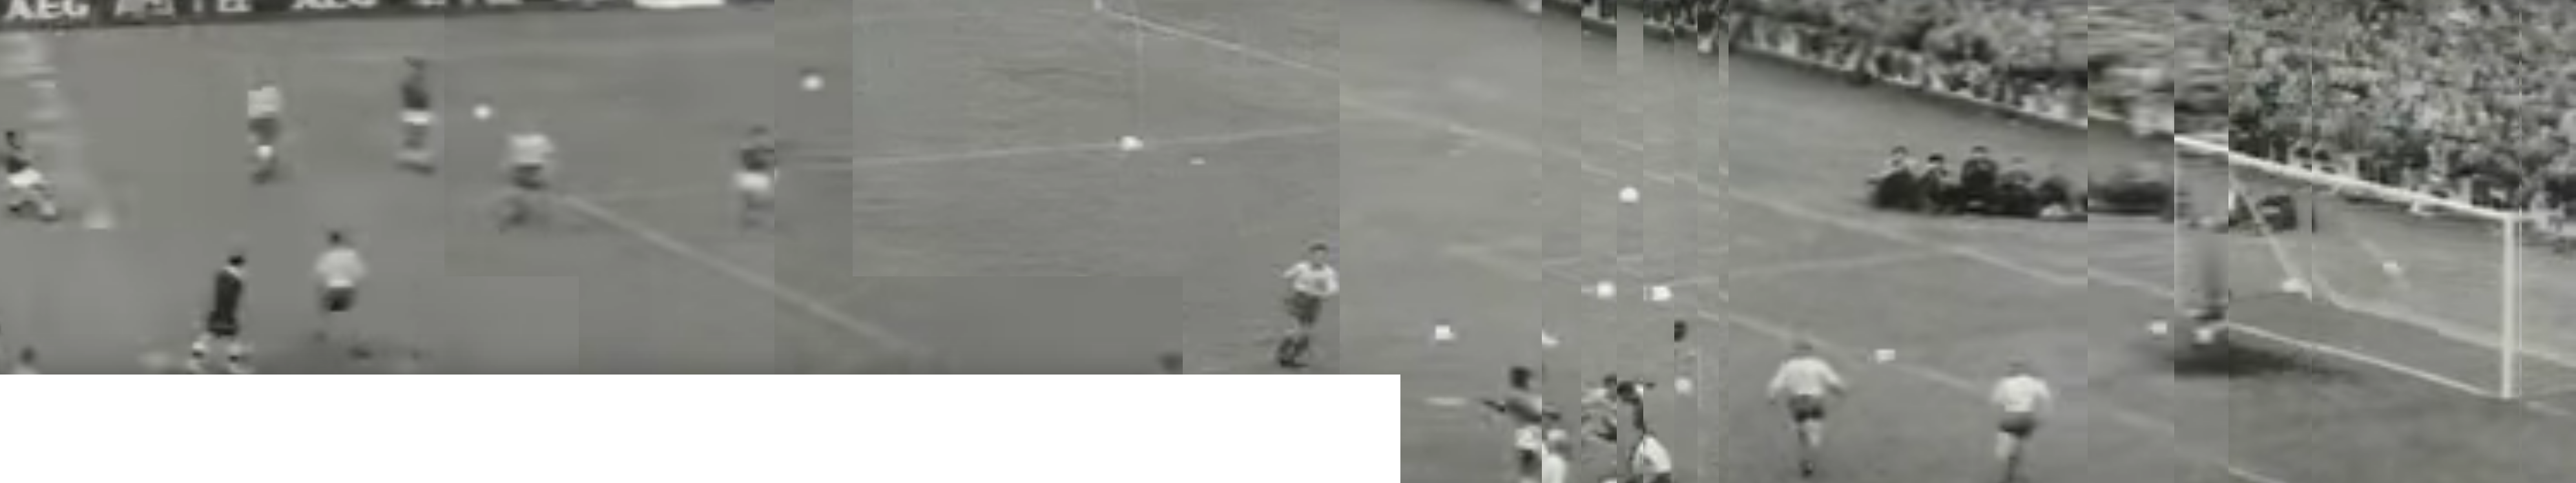
\includegraphics[width=\textwidth]{pele_goal}
\caption{Fonte: \url{https://www.youtube.com/watch?v=k1tKmCgF0sE}}
\end{figure}

A ideia, nessa imagem, é tentar traçar uma curva $S(x)$ que descreva
a trajetória da bola. Foram realizados três testes, cada um com quantidades
diferentes de pontos. A seguir, as curvas $S(x)$ para o gol do `Pelé':

\begin{figure}[H]
\centering
\includegraphics[width=\textwidth]{pele1}
\caption{Trajetória do gol do Pelé - 1. Pontos: \url{}}
\end{figure}

\begin{figure}[H]
\centering
\includegraphics[width=\textwidth]{pele2}
\caption{Trajetória do gol do Pelé - 2. Pontos: \url{}}
\end{figure}

\begin{figure}[H]
\centering
\includegraphics[width=\textwidth]{pele3}
\caption{Trajetória do gol do Pelé - 3. Pontos: \url{}}
\end{figure}

\section{Análise}

A implementação do método, assim como a maneira como é concebido,
é feita de forma muito mecânica e os algoritmos para a sua execução
não envolvem pensamentos computacionais complexos. Em todo o processo
de chegar às funções \textit{spline}, o pensamento matemático adotado
pelos autores de referência [1][3], ajudam a entender o porquê
das funções serem cúbicas e o porquê de algumas equações terem sido
adotadas durante a demonstração para as equações dos coeficientes
$a, b, c$ e $d$.

Como utilizamos o \textit{spline} natural, a resolução do sistema
linear encontrado é feita com um método iterativo, e durante
toda a implementação, a preocupação com o erro decorrente de
arredondamento foi desconsiderada, pois o objetivo do trabalho
é verificar se os splines oferecem uma boa aproximação para silhuetas.
Como se trata de uma interpolação, os valores presentes em um dado
intervalo não são conhecidos a priori, o que descarta a pretensão que
possa ser levantada em relação a um ajuste de curvas por outros métodos.

Um exemplo que ajuda a entender os resultados obtidos na seção anterior
é o da figura 12, o espectro do trecho de música. Os pontos que foram
utilizados para a interpolação estão muito próximos, mas mesmo assim
o método utilizou de funções cúbicas para o traçamento das curvas
$s_k(x)$. Isso mostra que, diferentemente de outros métodos de interpolação,
quanto mais pontos são fornececidos como referência para a curva $S(x)$, melhor
para a aproximação.

Nos outros dois exemplos, procuramos escolher apenas alguns pontos inicialmente
e aumentar a quantidade a fim de observar o comportamento da curva. Em ambos
as curvas melhoraram consideravelmente a aproximação da silhueta desejada.

Algo observado durante os testes, e que torna a implementação com o conceito
de conjuntos para os coeficientes muito útil, foi a diferença de espaçamento entre um
ponto e outro. Em funções que podemos escrever uma equação explícita, como
a usada na introdução, $f(x) = \frac{1}{x}$, quanto mais os pontos estiverem
igualmente espaçados, melhor para a curva gerada pelos \textit{splines}, pois
normalmente as derivadas seguem um padrão de crescimento e decrescimento.
Porém, em silhuetas, há mudanças bruscas tanto nos espaçamentos, quanto
nas inclinações das retas que podemos traçar entre dois pontos. Mesmo assim,
os \textit{splines} se adaptam a essas mudanças devido à preocupação
com as derivadas das próprias funções da curva.

\section{Conclusão}

Podemos dizer que o objetivo do trabalho foi alcançado, pois as implementações
propostas, juntamente com a demonstração do método levaram a boas
aproximações das silhuetas escolhidas pelo grupo.

Em um dos testes, um ponto foi colocado propositalmente à frente de outro,
com o objetivo de testar se era possível produzir uma curva que pudesse
ser intepretada como ``parametrizada'', apesar de estarmos apenas utilizando
valores de $x$ e $f(x)$. Como resultado, o método Gauss-Seidel não encontrou
solução para o sistema linear. Assim, um desafio (ou projeto) para o futuro
seria uma implementação de \textit{splines} para curvas paramétricas.

\begin{thebibliography}{9}

\bibitem{ruggiero}
RUGGIERO, M. A. G. E LOPES, V. L. R.
\textit{Cálculo numérico: aspectos teóricos e computacionais}, 2ª ed.
Pearson Makron Books, 1996.

\bibitem{artha}
GNU General Public License.
\textit{Artha ~ The Open Thesaurus}, version 1.0.3.
[Software]. Disponível em http://artha.sourceforge.net/wiki/.

\bibitem{burden}
BURDEN, R. L., E FAIRES, J. D.
\textit{Numerical Analysis}, 9ª ed.
Cengage Learning, 2011.

\end{thebibliography}



\end{document}
